\documentclass{ieeeaccess}
\usepackage{cite}
\usepackage{amsmath,amssymb,amsfonts}
\usepackage{algorithmic}
\usepackage{graphicx}
\usepackage{textcomp}
\usepackage{booktabs}
\usepackage{multirow}
\usepackage{subcaption}
\usepackage{bm}
\usepackage{float}
\makeatletter
\AtBeginDocument{\DeclareMathVersion{bold}
\SetSymbolFont{operators}{bold}{T1}{times}{b}{n}
\SetSymbolFont{NewLetters}{bold}{T1}{times}{b}{it}
\SetMathAlphabet{\mathrm}{bold}{T1}{times}{b}{n}
\SetMathAlphabet{\mathit}{bold}{T1}{times}{b}{it}
\SetMathAlphabet{\mathbf}{bold}{T1}{times}{b}{n}
\SetMathAlphabet{\mathtt}{bold}{OT1}{pcr}{b}{n}
\SetSymbolFont{symbols}{bold}{OMS}{cmsy}{b}{n}
\renewcommand\boldmath{\@nomath\boldmath\mathversion{bold}}}
\makeatother

\def\BibTeX{{\rm B\kern-.05em{\sc i\kern-.025em b}\kern-.08em
    T\kern-.1667em\lower.7ex\hbox{E}\kern-.125emX}}

%Your document starts from here ___________________________________________________
\begin{document}
\history{Date of publication xxxx 00, 0000, date of current version xxxx 00, 0000.}
\doi{10.1109/ACCESS.2024.0429000}

\title{Design and Evaluation of Multi-Agent Architectures
for Stock Price Prediction: A Vietnam Case Study}
\author{
    \uppercase{Duong Nguyen Minh}\authorrefmark{1}, 
    \uppercase{Dat Nguyen Huu}\authorrefmark{2}
}

\address[1]{Phenikaa School of Computing, Phenikaa University, Vietnam\\
(e-mail: 23010441@st.phenikaa-uni.edu.vn)}

\address[2]{Phenikaa School of Computing, Phenikaa University, Vietnam\\
(e-mail: dat.nguyenhuu@phenikaa-uni.edu.vn)}


\tfootnote{This paragraph of the first footnote will contain support
information, including sponsor and financial support acknowledgment. For
example, ``This work was supported in part by the U.S. Department of
Commerce under Grant BS123456.''}

\markboth
{Author \headeretal: Preparation of Papers for IEEE TRANSACTIONS and JOURNALS}
{Author \headeretal: Preparation of Papers for IEEE TRANSACTIONS and JOURNALS}

\corresp{Corresponding author: Duong Nguyen Minh (e-mail: 23010441@st.phenikaa-uni.edu.vn).}


\begin{abstract}
The Vietnamese stock has seen rapid expansion in
recent times; however, it is concurrently exhibiting increasing
volatility, and the methods employed by investors are getting
more complicated. Comprehending these evolving dynamics is
essential for formulating improved strategies and policies. This
research introduces a special simulation model designed for
Vietnam’s market, with six specialized agents, each contributes
a distinct and essential perspective — from trading behavior
and regulatory influence to financial performance analysis. To
examine coordination and decision mechanisms, three architectural designs are suggested:Hierarchical Architecture, modeling
top-down regulatory effects; Round Robin Architecture, ensuring equitable participation; and Ensemble Voting Architecture,
capturing collective consensus through decision aggregation.
By combining synthetic intelligence with agent-based modeling,
the model helps evaluate trading plans, market stability, price
changes, and how agents communicate. The results give new
insights into agent-to-agent interactions shaping market outcomes
and offer practical implications for the development of decisionsupport and regulatory assessment tools in emerging financial
systems such as Vietnam.

\end{abstract}

\begin{keywords}
Architectures, Multi-agent, Price Prediction, Viet Nam Stock
\end{keywords}

\titlepgskip=-21pt

\maketitle

\section{Introduction}
\label{sec:introduction}
The fast growth of digital technology in equity markets and the increasing availability of real-time market data  have created new chances for using artificial intelligence (AI) in trading and investment analysis. In Vietnam’s stock market, this change is especially relevant. By the end of 2024, there were about 9.3 million accounts for trading securities, with 99\% owned by domestic investors. Retail investors made up more than 80\% of all trade value \cite{theinvestor2025,vietnamnews2025,fiingroup2025}. These numbers show that Vietnam’s market is heavily driven by retail investors. It also shows that the market has high volatility, some inefficiencies, and a regulatory system that is still changing.

Traditional methods of equity-market analysis—technical analysis based on price patterns and fundamental analysis rooted in corporate disclosures—often struggle to capture the complex, non-linear relationships found in emerging markets. For instance, empirical evidence from Vietnam has revealed sluggish information dissemination, intraday trading frictions, and pronounced influences from investor sentiment and speculative behavior \cite{ha2025}. These characteristics underscore the limitations of conventional modelling approaches and reinforce the necessity for more adaptive and robust analytical frameworks.

Using deep learning setups with multi-agent systems presents a hopeful new way to deal with these challenges. Deep learning models can automatically extracting informative representations from large and complex datasets, thereby uncovering latent patterns and improving predictive accuracy. At the same time, multi-agent system designs let us simulate different market players and how they interact, offering a more realistic depiction of how markets work and how investors act.

To properly utilize AI-based strategies within Vietnam's stock market, it's essential to customize them carefully to align with its specific operational and conduct aspects. The primary issues includes data that is either disorganised or deficient, market behavior predominantly swayed by the sentiments of personal investors, and a legal and supervisory environment that constantly evolves and diverges from that of more mature economic systems. Therefore, combining complex analysis approaches with the unique features of the Vietnamese market is indispensable for unlocking the full potential of AI within this domain.

Accordingly, this study proposes a tailored simulation framework that combines specialised agent-modules and architectural designs to model Vietnamese stock-market dynamics. The focus will be on testing trading strategies, liquidity and volatility responses, and inter-agent communication under different coordination architectures. By doing so, the research contributes both to the academic understanding of agent-to-agent interactions in emerging markets and to the practical design of decision-support tools for Vietnam’s financial ecosystem.



\section{Literature Review}
\label{sec:Literature Review}

\subsection{Data Stock}
Data from worldwide stock exchanges has been acknowledged for a considerable period as a vital element for scholarly investigations and choices made by organizations. Established trading platforms like the NYSE, NASDAQ, LSE, and TSE function on a substantial level, having market values that go beyond USD 40–50 trillion when added up, and regular intraday trading volumes frequently go beyond hundreds of billions each day \cite{WorldFederation2024}. These marketplaces offer revisions to order books at the millisecond level, comprehensive limit order details (Level 3), and uniform high-frequency data streams appropriate for automated trading systems and studies into execution at the microsecond level \cite{Jones2019HFT}. These kinds of frameworks have paved the way for detailed studies of the structure of markets, latency-based arbitrage strategies, and how systemic risks extend throughout high-frequency settings.

In comparison, the stock market of Vietnam, which includes HOSE, HNX, and UPCoM, remains structurally smaller and data-constrained. The total value of all listed companies in 2024 is about USD 250–300 billion \cite{HOSE2024Report}, and the average value of daily trades is between USD 800 million and 1.2 billion, significantly lower than regional peers such as Thailand and Malaysia \cite{ADB2024}. Also, the data that is available is limited to the highest, lowest, opening, and closing prices at the end of the day, a summary of order flow, and recently, some basic looks at the order book, but it does not have timestamps measured in microseconds or complete insight into the depth of orders \cite{Nguyen2022Microstructure}. These limitations in structure show the general traits of markets that are still developing, which include bigger swings in returns, less involvement from big institutions, and more reaction to changes in rules and laws \cite{phan2015stock_khuong}.

A key behavioral divergence arises from the dominance of retail investors, who account for more than 85\% of total trading volume in Vietnam \cite{SSI2024Retail}. In contrast to markets run by big organizations where prices usually change based on news and profits, price changes in Vietnam tend to be more affected by government instructions, unofficial means of communication, and guesses based on feelings \cite{StateBank2023}. While markets around the world are starting to use news chosen by AI and different kinds of data in their trading systems \cite{BloombergAI2023}, what happens in the Vietnamese market is often influenced by what people feel on social media locally and what they think will happen with major government policies.

In conclusion, Vietnam stock market is not just a basic example of worldwide marketplaces; instead, it is a complex, emotionally reactive environment with a wide variety of behaviors, functioning with limited information, changing rules, and strong involvement from individual investors. This unique arrangement turns it into a fascinating place to test how well agent-based models and flexible AI systems work in developing economies.

\subsection{AI in Stock Price Prediction}

Over recent decades, artificial intelligence has advanced significantly in stock price prediction. Early studies focused on machine learning methods such as support vector machines, decision trees, random forests, and artificial neural networks, which captured non-linear relations between financial variables and returns and often outperformed statistical approaches \cite{kim2003,huang2005,patel2015}. Deep learning models like recurrent neural networks and long short-term memory further improved temporal analysis of financial time series \cite{fischer2018,chen2015}.

More recently, research has shifted toward \textit{Multi-Agent Systems} (MAS), where agents interact in simulated markets. Unlike traditional models treating prices as isolated data streams, MAS capture dynamic relations among traders, brokers, and regulators, enabling the study of phenomena such as herd behavior, bubbles, or irregularities \cite{lebaron2006,chen2012}. Combining reinforcement learning with agent-based simulations also deepens analysis of trading strategies, market stability, and inter-agent communication \cite{tesfatsion2006,wang2021}.

While the majority of MAS-based financial research has focused on mature markets such as the U.S. and China, empirical applications to emerging markets remain notably scarce. Regarding Vietnam, the AI-driven research currently available is mainly about price predictor trends over time via machine learning or deep learning techniques \cite{tran2020forecasting,pham2023lstm}, without regard for the ways that actions driven by individual investors, governmental policy shifts, or sudden shifts in general attitudes can shape the market. These influences have been observed in empirical studies to affect how prices are set in the Vietnamese equity market \cite{phan2015stock_khuong}. This highlights the necessity of Multi-agent frameworks that capable of simulating Vietnam’s unique market environment rather than merely predicting price trajectories. 

Overall, this shift from single-model learning to multi-agent simulation reflects a growing recognition of stock markets as complex ecosystems shaped by interactions among diverse actors. This approach provides a useful means to examine regulatory effects and investor behavior in experimental settings, particularly relevant for developing economies like Vietnam.

\subsubsection{Machine Learning for Stock}
The utilization of machine learning methodologies has been a long-standing practice in stock price prediction, non-linear trends within the realm of financial time series data. An illustrative example is seen in Kim \cite{kim2003}, where support vector machines (SVM) were employed to project the fluctuations in the stock market, achieving a level of effectiveness that surpassed that of conventional statistical modeling techniques. Similarly, Huang et al. \cite{huang2005} used the capabilities of SVM to forecast the directional prediction of stock indices, whereas Patel et al. \cite{patel2015} made use of a hybrid of artificial neural networks (ANN), random forests, and SVM, all in pursuit of heightened predictive precision. Progressing into more contemporary research, there has been an assimilation of deep learning techniques, notably the adoption of long short-term memory (LSTM) models, which possess the inherent capacity to discern temporal interrelationships within sequences of prices \cite{fischer2018,chen2015}.

Generally, these types of models use structured data such as past prices, amount of trading, and market measures as well as sometimes unstructured data like news or feelings on social media and then give either a price prediction or where the market is likely to go, whether up or down. Although the results frequently demonstrate better accuracy than standard statistical comparisons, there are still some problems. Initially, machine learning models can easily become too overfitting to the data in fast-changing markets where patterns are unstable. Secondly, they mostly view the market as a simple system where data goes in and results come out, ignoring how investors change and affect each other. Finally, these models have difficulty clarifying new events like market booms, collapses, or sudden drops in trading because these come from group actions rather than single pieces of information.

To solve these challenges, researchers have suggested moving towards \textit{Multi-Agent Systems} (MAS). Multi-Agent Systems, in contrast to traditional machine learning, clearly represent multi agents, such as investors, brokers, and regulators, who interact under market rules and adapt their strategies over time. This allows for the analysis of complex, emergent behaviors beyond prediction accuracy, offering more thorough knowledge of market stability, widespread dangers, and the significance of agent communication \cite{lebaron2006,chen2012,tesfatsion2006,wang2021}. From this perspective, Multi-Agent Systems do not merely complement traditional machine learning, but extend it by embedding predictive intelligence into an interactive and behaviorally realistic market environment — a setup particularly well-suited to Vietnam’s retail-dominated and sentiment-driven stock market structure..

\subsubsection{Multi-Agent for Stock Price Prediction}
Initial uses of Multi-Agent Systems in the world of finance were primarily aimed at mirroring how markets behave, instead of trying to predict what prices would be. Groundbreaking research, like the work done by LeBaron \cite{lebaron2006} and Tesfatsion \cite{tesfatsion2006}, revealed that different agents working together can recreate typical market behaviors, such as prices changing a lot in short periods or market bubbles. These are trends that standard statistical analysis or single-model learning methods fail to explain.
Subsequent projects took MAS a step further into areas where agents could learn and improve their trading skills through trial and error. As an example, Chen et al. \cite{chen2012} highlighted how unexpected market behaviors can arise, and Wang et al. \cite{wang2021} were able to create investment portfolios that did better than those that followed fixed, unchanging rules.

Recent MAS research are increasingly focusing on  hybrid learning-based architectures, where automated systems communicate and also forecast prices using artificial market settings. These approaches better reflect real trading behavior , flexible outlooks, and changing risk attitudes, these strategies offer a superior depiction of actual trading actions, exceeding simple historical trend analysis.

\section{Methodology}
\subsection{Architectural Overview}
The proposed Multi-Agent System (MAS) represents a sophisticated computational framework designed to address the unique challenges of stock price prediction in Vietnam's emerging market environment. The system integrates six specialized autonomous agents, each equipped with domain-specific analytical capabilities, operating within three distinct coordination architectures to deliver robust and interpretable financial forecasts. At its core, the system employs a foundation layer built upon \textbf{Long Short-Term Memory (LSTM)} networks to capture temporal dependencies in historical price data, enhanced through the coordinated intelligence of specialized agents covering technical analysis, fundamental evaluation, risk assessment, sentiment processing, and market microstructure analysis.

The cognitive intelligence of the system is powered by \textbf{Google Gemini} as the core Large Language Model (LLM), selected for its exceptional scalability, low-latency execution, and expansive context window capabilities essential for processing complex financial narratives and multi-dimensional market data. The system's architectural flexibility is demonstrated through three coordination paradigms—\textbf{Hierarchical, Round Robin, and Ensemble Voting architectures}—each specifically calibrated to handle Vietnam's market characteristics, including the T+2.5 settlement period, 85-90\% retail investor dominance, and pronounced sentiment-driven volatility, delivering predictions across short-term (3 days), medium-term (14 days), and long-term (60 days) investment horizons.

\begin{figure}[H]
    \centering
    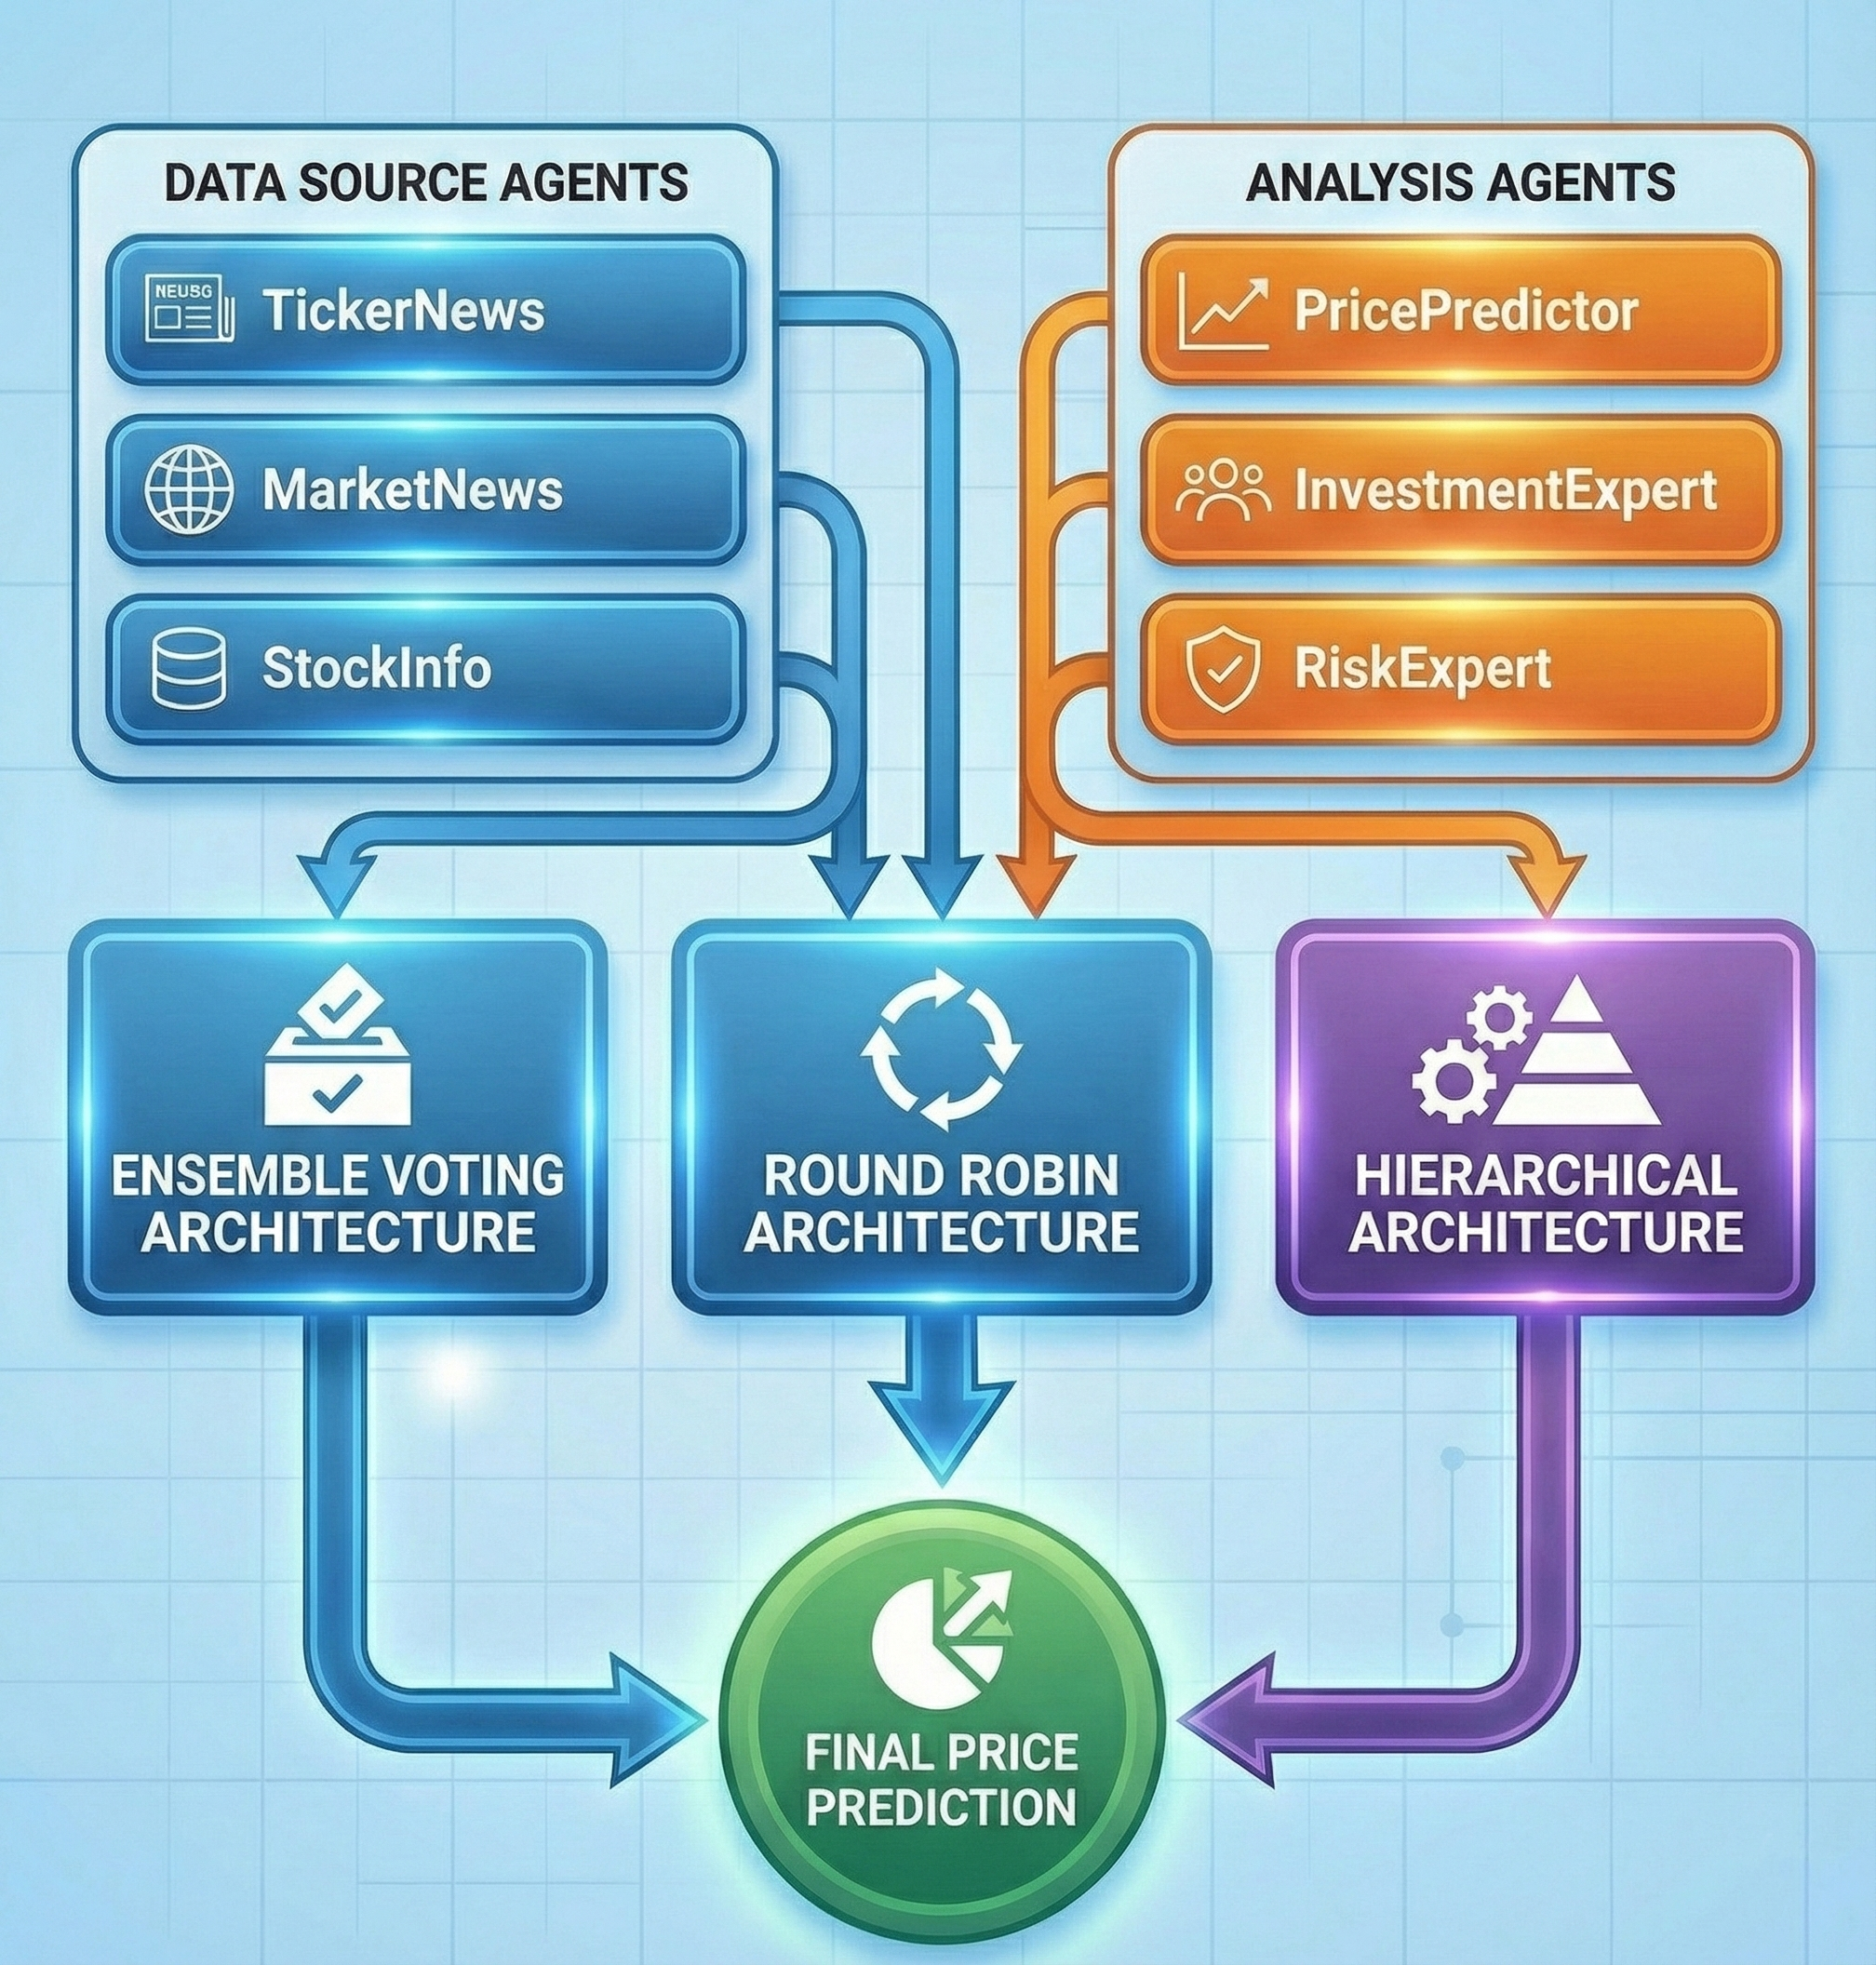
\includegraphics[width=0.9\linewidth]{anh/overrall11.png}
    \caption{
System overview diagram}
    \label{fig:
System overview diagram}
\end{figure}

\subsection{The Specialized Agent Team}
\subsubsection{Agents Overview}
\begin{itemize}
    \item \textbf{PricePredictor Agent:} 
    Uses the primary LSTM forecast blended with technical tools just like the \textbf{Relative Strength Index (RSI)}, \textbf{Moving Average Convergence Divergence (MACD)}, and \textbf{Bollinger Bands}. By analyzing tendencies and momentum, it improves the starting predict to offer a greater correct rate prediction together with a confidence rating for the technical analysis.

    \item \textbf{InvestmentExpert Agent:} 
    InvestmentExpert Agent: Takes into consideration critical financial numbers which include the \textbf{Price-to-Earnings ratio (P/E)}, \textbf{Price-to-Book ratio (P/B)}, \textbf{Return on Equity (ROE)}, \textbf{Earnings Per Share growth (EPS)}, and \textbf{Debt-to-Equity ratio}. It plays an intensive assessment of the company`s financial health and growth potential, ensuing in a proposal to both \textbf{BUY, SELL, or HOLD}, together with a confidence score for its financial analysis.

    \item \textbf{RiskExpert Agent:} 
    Analyzes volatility profiles, marketplace correlation matrices, and historical drawdown data. It evaluates general portfolio risk via volatility modeling and correlation dynamics, offering a quantified risk stage with corresponding position sizing guidance.

    \item \textbf{TickerNews Agent:} 
    Processes company-specific news sourced from systems including CafeF, VietStock,... and earnings releases. Employing sentiment classification and event-driven effect evaluation, it outputs a sentiment polarity rating coupled with an expected marketplace effect magnitude.

    \item \textbf{MarketNews Agent:} 
    Examines macroeconomic updates, marketplace sentiment data, and valuable bank communications. Through systemic threat evaluation and regime classification, it generates a contextual marketplace rating reflecting prevailing macroeconomic conditions.

    \item \textbf{StockInfo Agent:} 
    Analyzes trading volume, liquidity trends, and technical metadata to assess marketplace microstructure. The agent presents a liquidity-adjusted feasibility score followed through execution-related suggestions for most reliable trade deployment.
\end{itemize}

\subsubsection{LLMs Overview}
In this study, \textbf{Google Gemini 2.0 Flash} is selected as the core LLM due to its high scalability, low-latency cloud execution, and exceptionally large context window, making it well-suited for production-grade AI pipelines. To provide a broader comparative perspective, we additionally include \textbf{OpenAI GPT-4o} and \textbf{Llama-3.1-70B-Instruct-Turbo}. GPT-4o is recognized for its strong reasoning quality and balanced multimodal performance, whereas Llama-3.1 offers significant advantages for privacy-focused and offline deployments. The operational characteristics of these models are summarized in Table~\ref{tab:llm_comparison_summary_en}.

\begin{table}[h!]
\centering
\caption{Operational Characteristics and Execution Behavior of Leading Large Language Models.}
\label{tab:llm_comparison_summary_en}
\resizebox{\columnwidth}{!}{
\begin{tabular}{@{}lccc@{}}
\toprule
\textbf{Criterion} & \textbf{Gemini 2.0 Flash} & \textbf{GPT-4o} & \textbf{Llama-3.1-70B} \\ \midrule
Deployment & Cloud API & Cloud API & Local / Hosted \\
Latency & Low & Medium & Low / Variable \\
Throughput & Very High & High & Infra-dependent \\
Offline Capability & None & None & Yes \\
Context Window & Up to 1M tokens & Up to 128k tokens & Model-dependent \\
Cost Model & SaaS (usage-based) & SaaS (usage-based) & CapEx / SaaS \\
Optimized for & Cloud scale & Reasoning quality & Privacy / Control \\ 
\bottomrule
\end{tabular}
}
\end{table}

\subsection{Coordination Architectures}
\subsubsection{Hierarchical Architecture (Design 1)}

\paragraph{Operational Mechanism}
The hierarchical architecture operates under a Master–Subordinate coordination paradigm, in which a single centralized \textit{Master Agent} oversees six \textit{Specialized Agents}, each responsible for processing distinct streams of financial information, including technical indicators, fundamental metrics, portfolio risk profiles, market sentiment, and microstructure data. Each agent functions independently and in parallel, enabling efficient handling of heterogeneous inputs while preserving modular expertise. The \textit{Master Agent} then collects and consolidates all outputs, performing rigorous consistency checks and employing ensemble synthesis techniques to generate a unified, coherent market prediction that reflects multiple analytical perspectives, thereby enhancing reliability, robustness, and interpretability. This design balances computational efficiency with structured integration of diverse financial insights, allowing disparate information sources to interact within a centralized decision-making framework that supports scalable, actionable, and interpretable outcomes. Similar hierarchical coordination principles have been successfully applied in multi-agent financial simulations to improve decision consistency and system scalability~\cite{tesfatsion2006,lebaron2006}.
\\
Furthermore, maintaining modularity at the agent level enables targeted refinement and adaptive learning within individual analytical domains, progressively enhancing predictive accuracy. This multi-layered coordination approach supports robust ensemble predictions while providing a transparent framework to trace each analytical stream’s contribution to the final market decision, thereby reinforcing interpretability and trustworthiness in complex financial environments.

\begin{figure}[H]
    \centering
    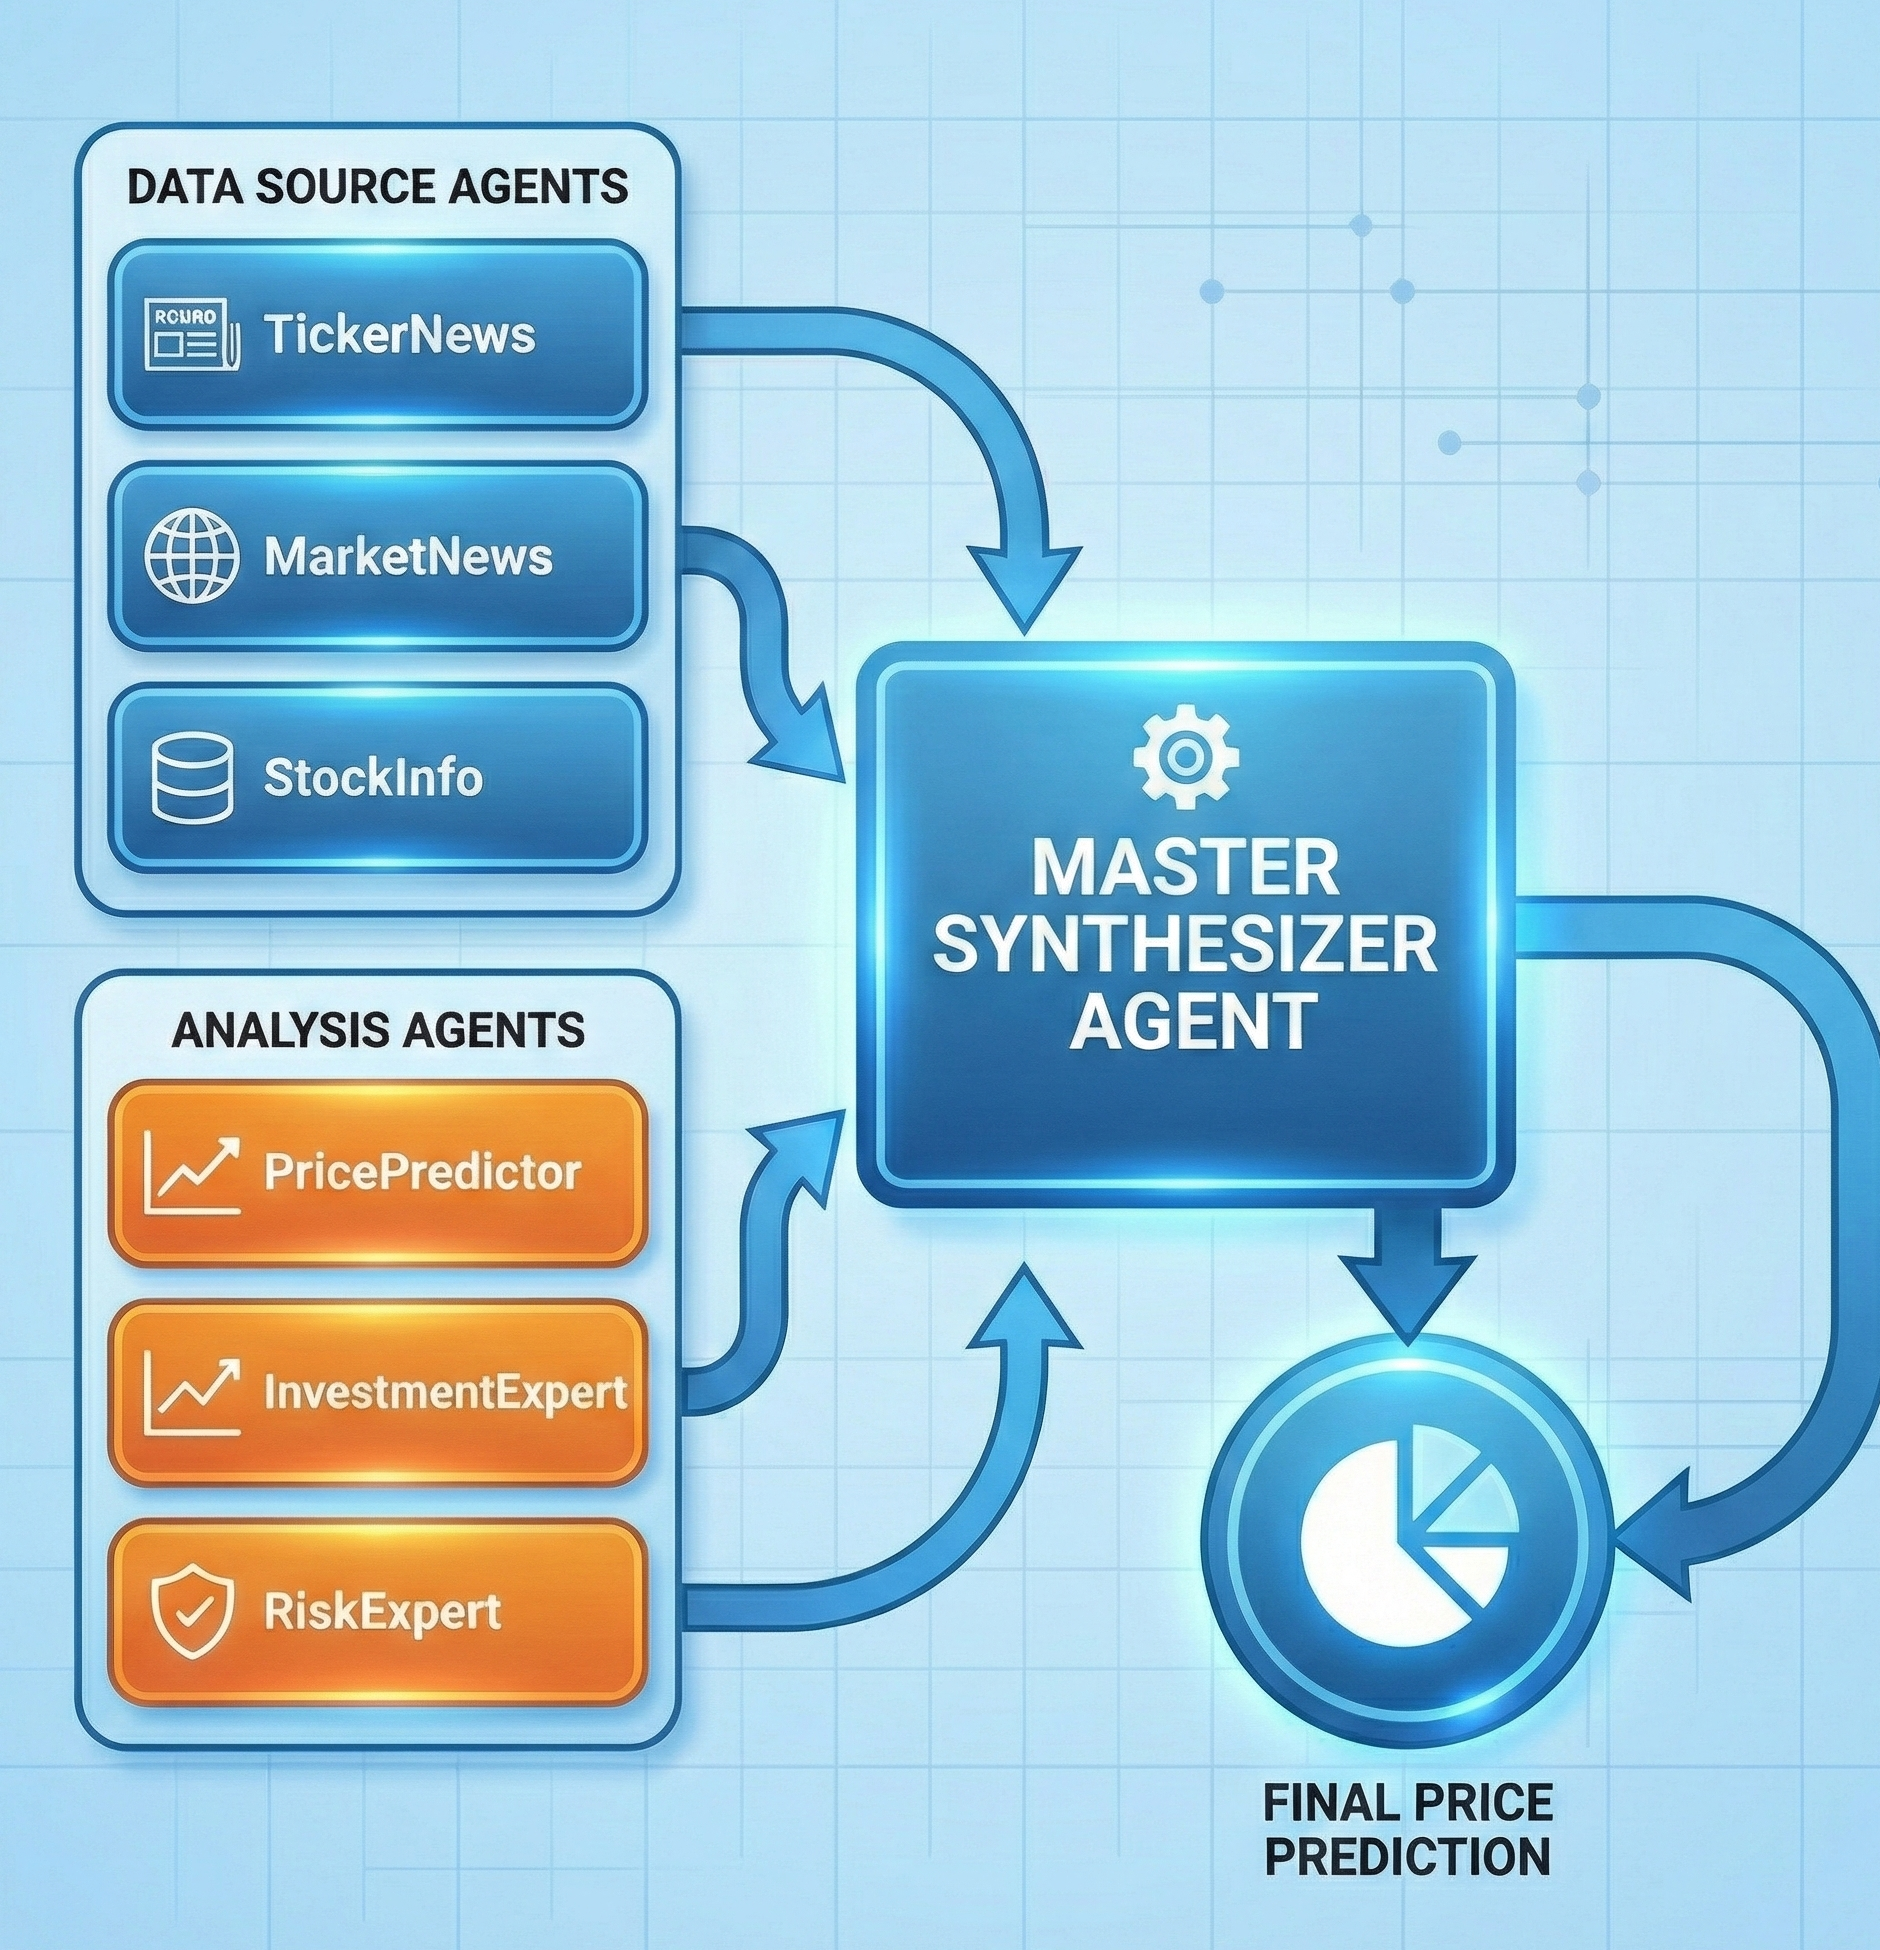
\includegraphics[width=0.9\linewidth]{anh/hie3.png}
    \caption{Hierarchical architecture with a Master Agent coordinating six specialized agents. Each agent processes domain-specific data in parallel, and the Master Agent aggregates outputs for final prediction.}
    \label{fig:hierarchical_architecture}
\end{figure}


\paragraph{Workflow}
The hierarchical architecture operates through a structured sequence of five key stages:

\begin{enumerate}
    \item \textbf{Data Acquisition and Preprocessing} — 
    The system collects and preprocesses multi-source financial data, including technical indicators, fundamental ratios, and market sentiment signals.
    
    \item \textbf{LSTM Foundation Modeling} — 
    An LSTM-based model generates the initial price prediction, serving as the base signal for subsequent multi-agent analysis.
    
    \item \textbf{Parallel Agent Processing} — 
    Six specialized agents operate simultaneously, each focusing on a distinct analytical dimension such as risk assessment, fundamental valuation, and news sentiment interpretation.
    
    \item \textbf{Master Agent Aggregation} — 
    The Master Agent consolidates all intermediate outputs, performing validation and consistency checks to ensure model reliability and coherence.
    
    \item \textbf{Final Output Generation} — 
    The system produces the unified result, including final price forecasts, confidence levels, and investment recommendations.
\end{enumerate}

\subsubsection{Round Robin Architecture (Design 2)}
\paragraph{Operational Mechanism}
The Round Robin architecture follows a sequential refinement process, in which every agent gets the output from the former stage, improves it by the use of its specialized analysis, and passes it forward. This iterative chain allows modern development of predictions via multi-perspective evaluation \cite{wang2021,tesfatsion2006,lebaron2006,chen2012}. 


\begin{figure}[H]
    \centering
    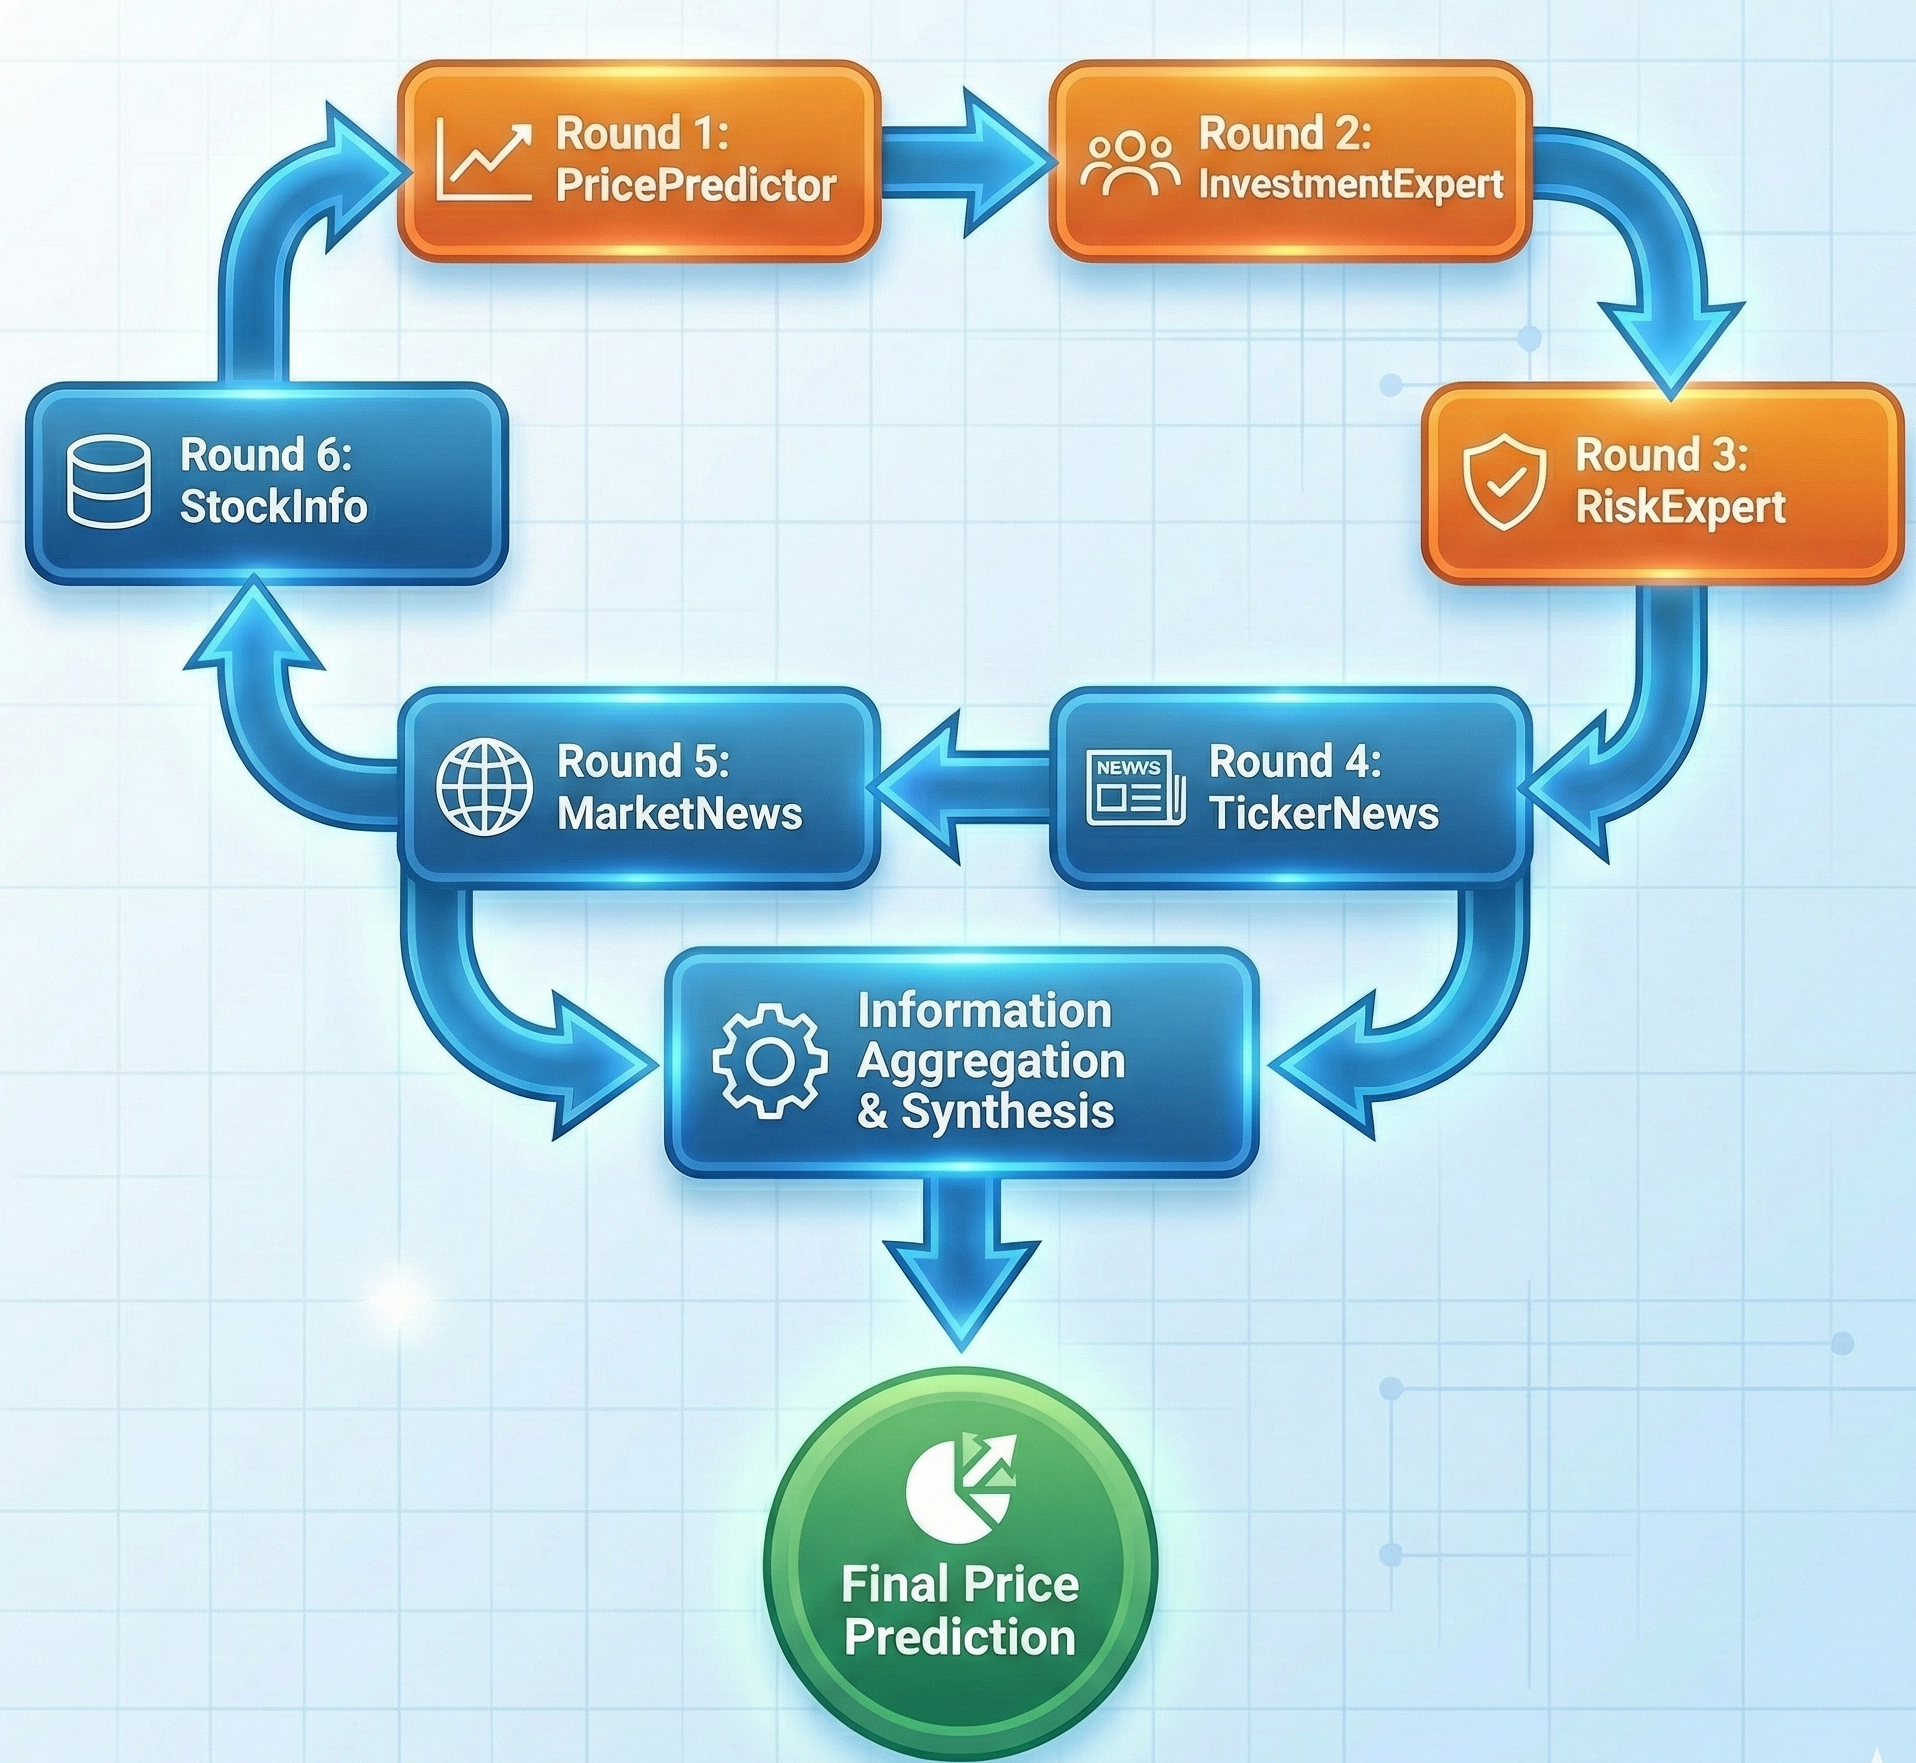
\includegraphics[width=0.9\linewidth]{anh/rr4.png}
    \caption{Round Robin architecture with six specialized agents operating in a sequential refinement cycle.}
    \label{fig:hierarchical_architecture}
\end{figure}



\paragraph{Workflow} The round robin operates via an organized sequence of a few steps:

\begin{enumerate}
    \item \textbf{Initialization.} The approach begins with the  \textit{LSTM Foundation Layer}, which constructs the initial predictive state by capturing temporal dependencies in the historical data. This state serves due to the fact that the baseline representation of the market dynamics before any domain-specific refinement is applied.  

    \item \textbf{Sequential Agent Flow.} The predictive state is propagated through six specialized agents in a fixed order: Round~1 $\rightarrow$ Round~2 $\rightarrow$ Round~3 $\rightarrow$ Round~4 $\rightarrow$ Round~5 $\rightarrow$ Round~6. Each agent operates as a refinement node, sequentially receiving the previous output, performing its own analysis, and forwarding an improved result to the subsequent stage.  

    \item \textbf{Incremental Enhancement.} Within this Round Robin structure, every agent contributes a unique perspective—technical, fundamental, risk-based, news-driven, or macroeconomic—to enrich the evolving state. This iterative enhancement ensures that both micro-level indicators and macro-level contexts are systematically embedded into the prediction pipeline.  

    \item \textbf{Decision Traceability.} Throughout the refinement sequence, all intermediate states and analytical decisions are logged to preserve a transparent audit trail. This traceability allows researchers and practitioners to examine how individual agents influenced the outcome, thereby supporting interpretability and trust in model-driven recommendations.  

    \item \textbf{Cumulative Refinement Output.} Upon completion of the six-round iteration, the framework consolidates the results into a final state representing the cumulative learning and multi-perspective reasoning of the entire agent ensemble. The resulting output thus reflects not only predictive accuracy but also contextual awareness and adaptive decision integration across the full refinement cycle.  
\end{enumerate}

\subsubsection{Ensemble Voting Architecture (Design 3)}
\paragraph{Operational Mechanism}
The Ensemble Voting Architecture employs an intelligent voting system in which six separate agents work at the same time and on their own. Every agent carries out focused studies on different data fields, which ensures that a wide range of predictive angles are taken into account. After this, the system uses a statistical inference engine to combine these findings. This engine makes use of dynamic weighting according to the recent performance, execution time, and confidence score. This versatile strategy improves robustness and reduces bias, facilitating more dependable and easily understood collective predictions within financial predictions~\cite{opera2023}.

\begin{figure}[H]
    \centering
    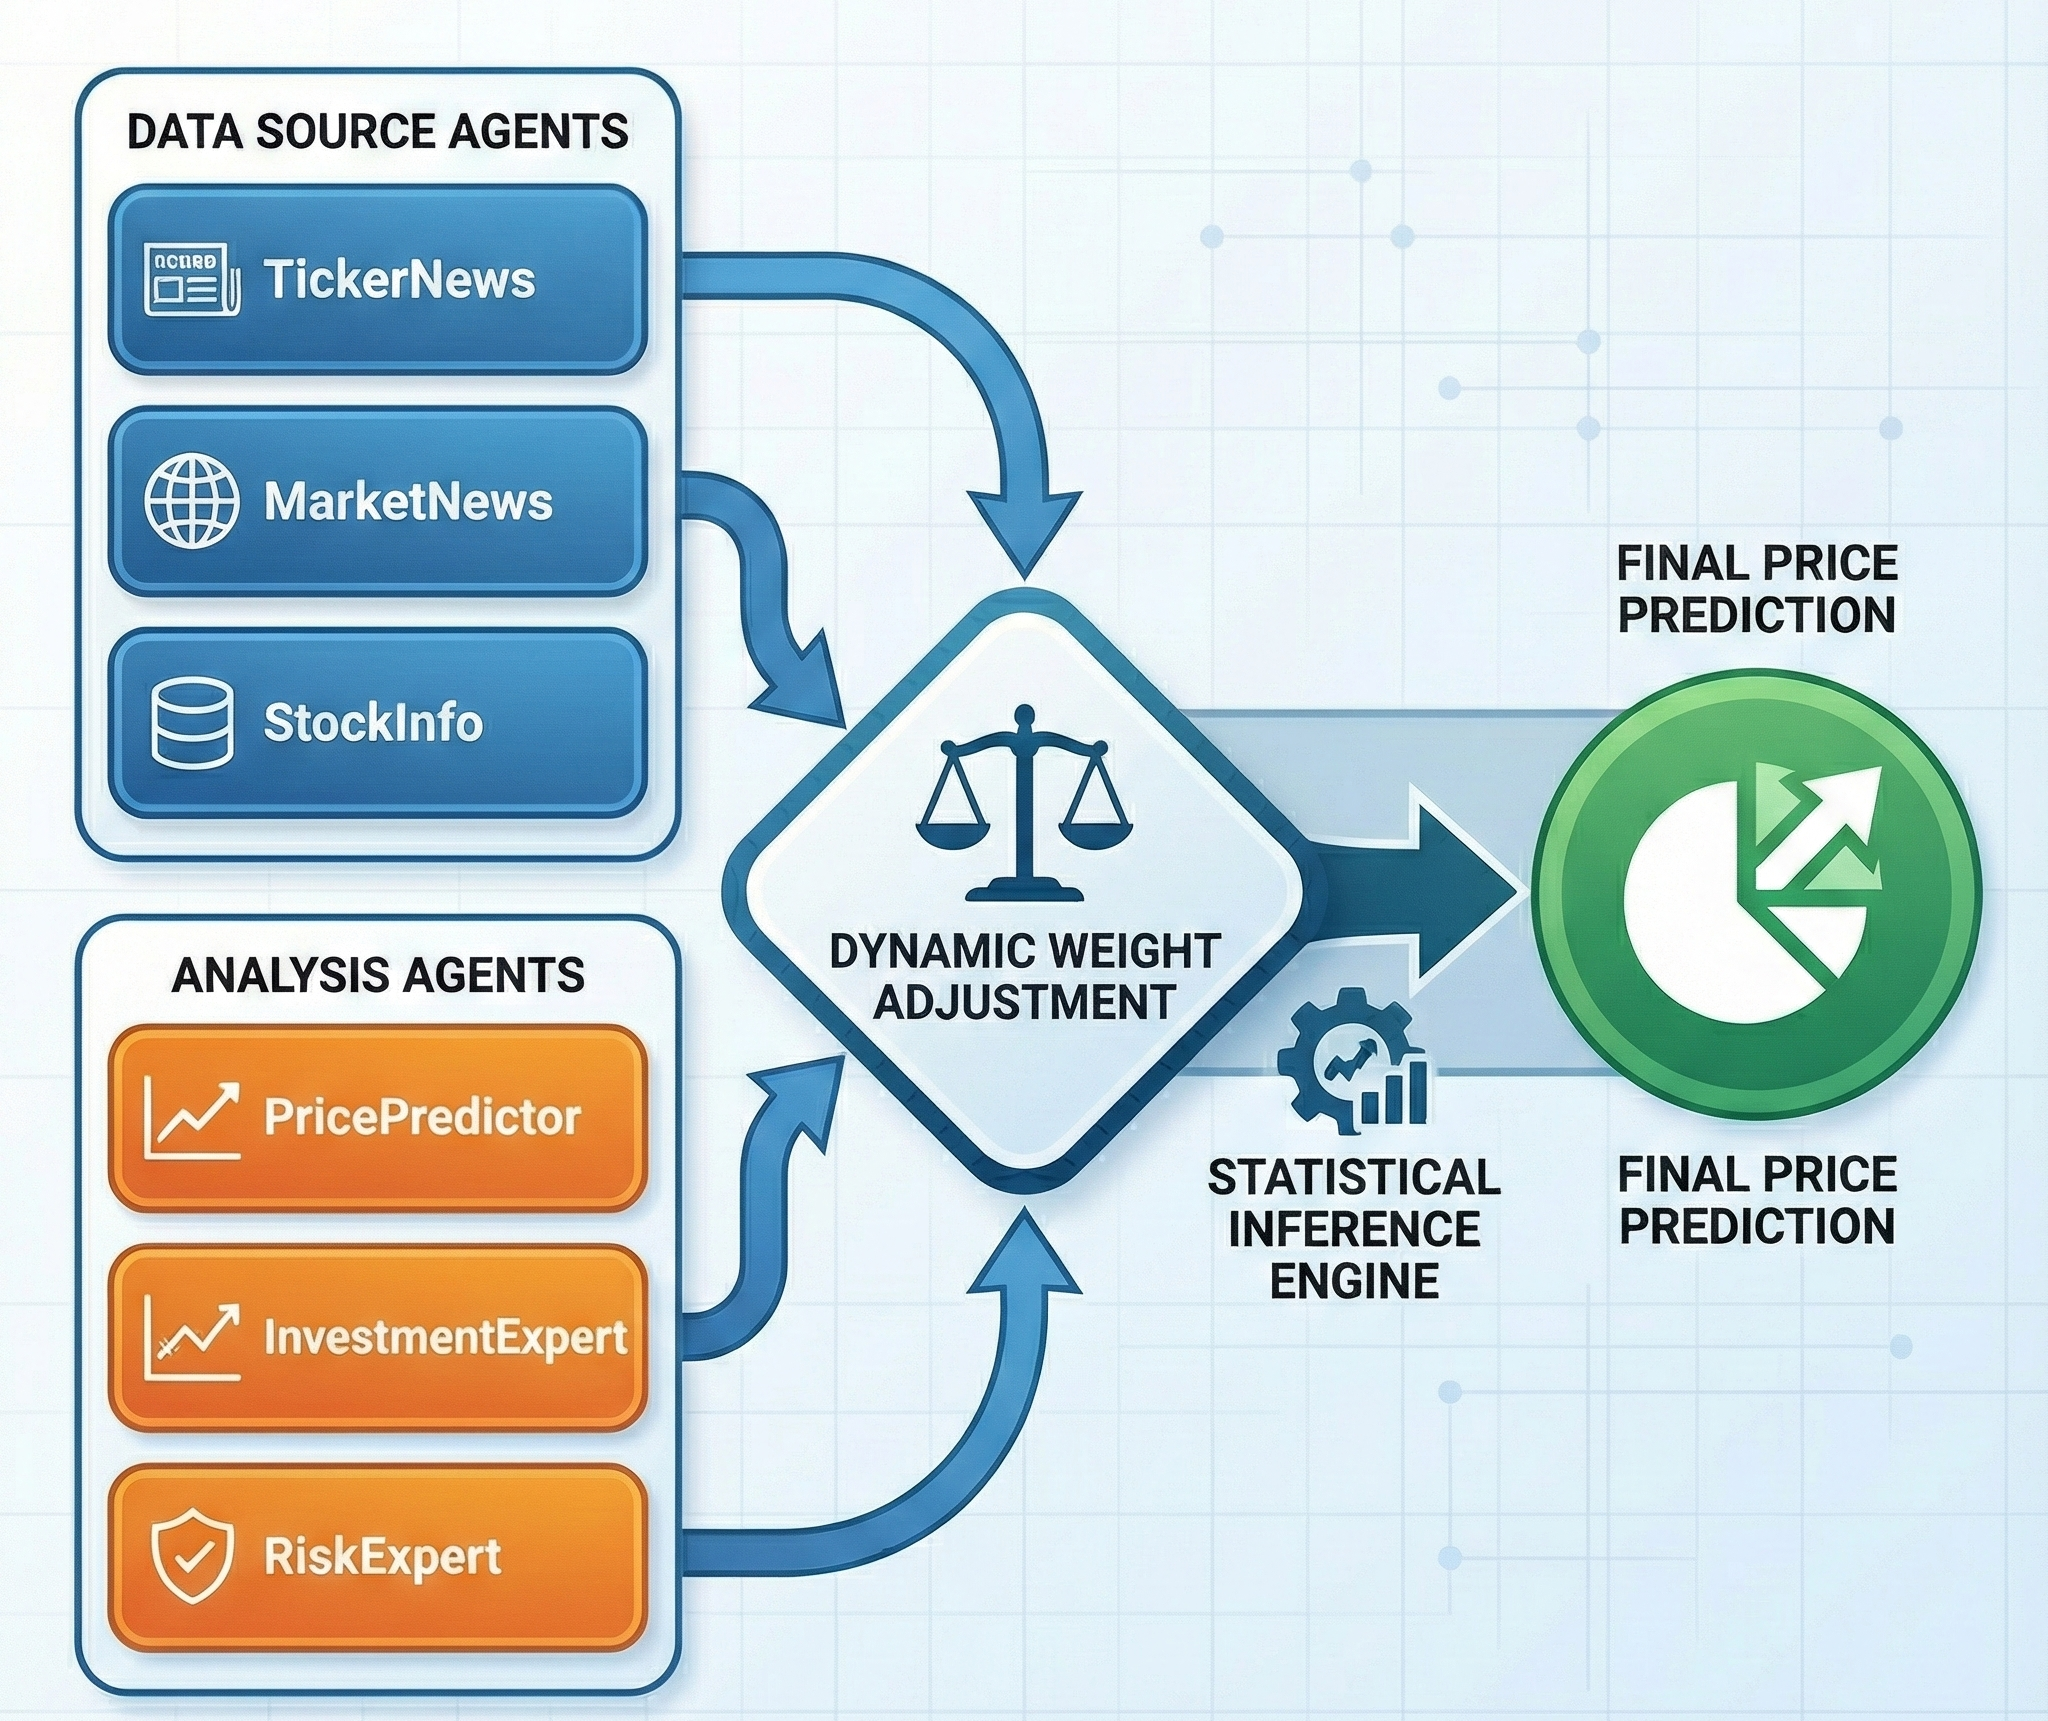
\includegraphics[width=0.9\linewidth,height=8cm]{anh/em4.png}
    \caption{Ensemble Voting Architecture  with six specialized agents employing an intelligent voting }
    \label{fig:hierarchical_architecture}
\end{figure}


\paragraph{Workflow}
The operational flow of the proposed Ensemble Voting Architecture is summarized as follows:

\begin{enumerate}
    \item \textbf{Data Distribution:} Input data streams are concurrently distributed to all six agents.
    \item \textbf{Parallel Processing:} Each agent operates independently in parallel, ensuring full task isolation.
    \item \textbf{Performance Evaluation:} Real-time assessment of individual agent performance is continuously conducted.
    \item \textbf{Dynamic Weight Adjustment:} Model weights are adaptively updated based on the latest performance metrics.
    \item \textbf{Statistical Inference Integration:} Final aggregation is performed through statistical inference with uncertainty quantification to enhance predictive reliability.
\end{enumerate}




\paragraph{Dynamic Weight Adjustment Process}
To maintain adaptiveness in a volatile environment, the model employs a continuous weight adjustment mechanism.  
First, each agent’s recent performance is evaluated through multiple metrics including prediction accuracy, confidence calibration, and execution latency.  
Second, agent weights are updated proportionally to recent efficiency, ensuring that higher-performing agents exert greater influence.  
Third, normalization is applied to maintain a total ensemble weight of unity.  
Lastly, real-time optimization enables the system to react dynamically to shifting market conditions, preserving robustness and responsiveness over time.\cite{McAndrew2021,Lu2023}

\paragraph{Statistical Inference Process}
The ensemble layer integrates all agent outputs through a statistically grounded inference procedure.  
Predictions are first aggregated using dynamically adjusted weights to produce a composite forecast.  
Uncertainty quantification is then conducted via variance estimation to assess reliability.  
Consensus analysis measures inter-agent agreement, capturing alignmente across diverse analytical dimensions.  
Finally, statistical validation is performed to verify the ensemble’s internal coherence and predictive soundness, ensuring that aggregated outputs remain both consistent and interpretable in empirical contexts (see e.g., \cite{wang2021,li2022}). 






\section{Empirical Evaluation}
\subsection{Research Questions (RQs)}
To rigorously assess the effectiveness of our proposed framework, \textsc{Multi-Agent Viet Nam Stock}, we design our empirical study around the following research questions:

\textbf{RQ1. [Coordination Effectiveness]}  
Which coordination architecture (Hierarchical, Round Robin, or Ensemble) is the most effective for the Vietnamese stock market?

\textbf{RQ2. [Multi-Agent vs. Single-Agent Architectures]}  
Does the Multi-Agent system outperform traditional Single-Agent (LSTM) models?


\subsection{Dataset \& Settings}
A fundamental structural characteristic of the Vietnamese stock market is its \textbf{T+2.5 settlement period}. Given that \textit{domestic individual investors overwhelmingly dominate the market, accounting for approximately 85-90\% of daily trading value} \cite{TinNhanhChungkhoan2025}, this configuration strongly incentivizes rapid, short-term speculative trading. This retail-heavy structure, often characterized by significant \textit{herd behavior} rather than fundamental analysis, is identified by analysts as a primary driver of the market's notoriously high price volatility \cite{WorldBank2024, Yuanta2025}.



Inspired by the substantial effects of this behavioral pattern, the current research undertakes a sector-specific analysis focusing on four key areas of the Vietnamese economy: \textbf{Banking(VCB)}, \textbf{Technology(FPT)}, \textbf{Real Estate(DXG)}, and \textbf{Industrial Construction(VCS)}.


To rigorously evaluate predictive performance across heterogeneous investment horizons, the 
analysis is structured into three temporal regimes:
\begin{itemize}
    \item \textbf{Short-term (3 days):} aligned with the T+2.5 settlement window, capturing immediate speculative turnover.
    \item \textbf{Medium-term (14 days):} representing a conventional tactical positioning horizon.
    \item \textbf{Long-term (60 days):} proxying strategic buy-and-hold investment behavior.
\end{itemize}

To ensure robustness and reduce temporal bias, the evaluation at each forecasting horizon (\textbf{Short-term}, \textbf{Medium-term}, \textbf{Long-term}) is conducted across four distinct market intervals:
\begin{enumerate}
    \item \textbf{Late August to early September}: capturing post-summer liquidity shifts;
    \item \textbf{16/10/2025}: representing a period of heightened trading activity;
    \item \textbf{21/10/2025}: corresponding to a stabilization phase after short-term volatility;
    \item \textbf{22/10/2025}: reflecting market behavior during an immediate rebound window.
\end{enumerate}
Assessing performance across these four checkpoints enables a comprehensive examination of model behavior under varying liquidity, volatility, and sentiment conditions, thereby strengthening the validity of comparative results across all three time horizons.


\subsection{Evaluation Metrics.} 
To rigorously evaluate the predictive performance of the proposed framework, this study utilizes three established statistical indicators: Mean Absolute Error (MAE), Root Mean Square Error (RMSE), and Mean Absolute Percentage Error (MAPE). MAE quantifies the average magnitude of errors in a set of forecasts without considering their direction, providing a linear score that weights all individual differences equally~\cite{willmott2005advantages}. Conversely, RMSE operates as a quadratic scoring rule; by squaring residuals prior to averaging, it assigns greater weight to larger deviations, thereby increasing sensitivity to outliers~\cite{chai2014root}. Finally, MAPE measures accuracy as a relative percentage, facilitating the comparison of forecasting performance across datasets with differing scales~\cite{hyndman2006another}.

\section{Coordination Effectiveness (RQ1)}
This section addresses the first research question regarding the comparative effectiveness of the three proposed multi-agent architectures: Hierarchical, Round Robin, and Ensemble Voting. To evaluate their adaptability to the high volatility characteristic of the Vietnamese market, we analyzed predictive performance across three distinct time horizons.

\subsection{Results of Short-term}
This horizon closely reflects the microstructural dynamics surrounding the T+2.5 settlement cycle, where short-lived price movements are driven primarily by liquidity shocks, rapid position unwinding, and speculative round-trip trades. As such, the 3-day window provides a focused setting to evaluate each model’s ability to track high-frequency sentiment shifts and transient order-flow imbalances that typically dissipate before fundamentals exert meaningful influence.


\section{Multi-Agent vs. Single-Agent (RQ2)}
Below figures illustrate the results obtained for four selected stocks—DXG, FPT, VCB, and VCS—when analyzed individually using a single-agent approach based solely on the core LSTM model. Each subplot highlights the predictive performance for the corresponding stock, providing a clear visualization of the medium-term price dynamics captured by the model. This setup emphasizes the capability of the LSTM as a standalone agent to extract temporal patterns and generate actionable forecasts across different equities.

\begin{figure}[H]
    \centering
    % Hàng 1
    \begin{subfigure}[b]{0.48\columnwidth}
        \centering
        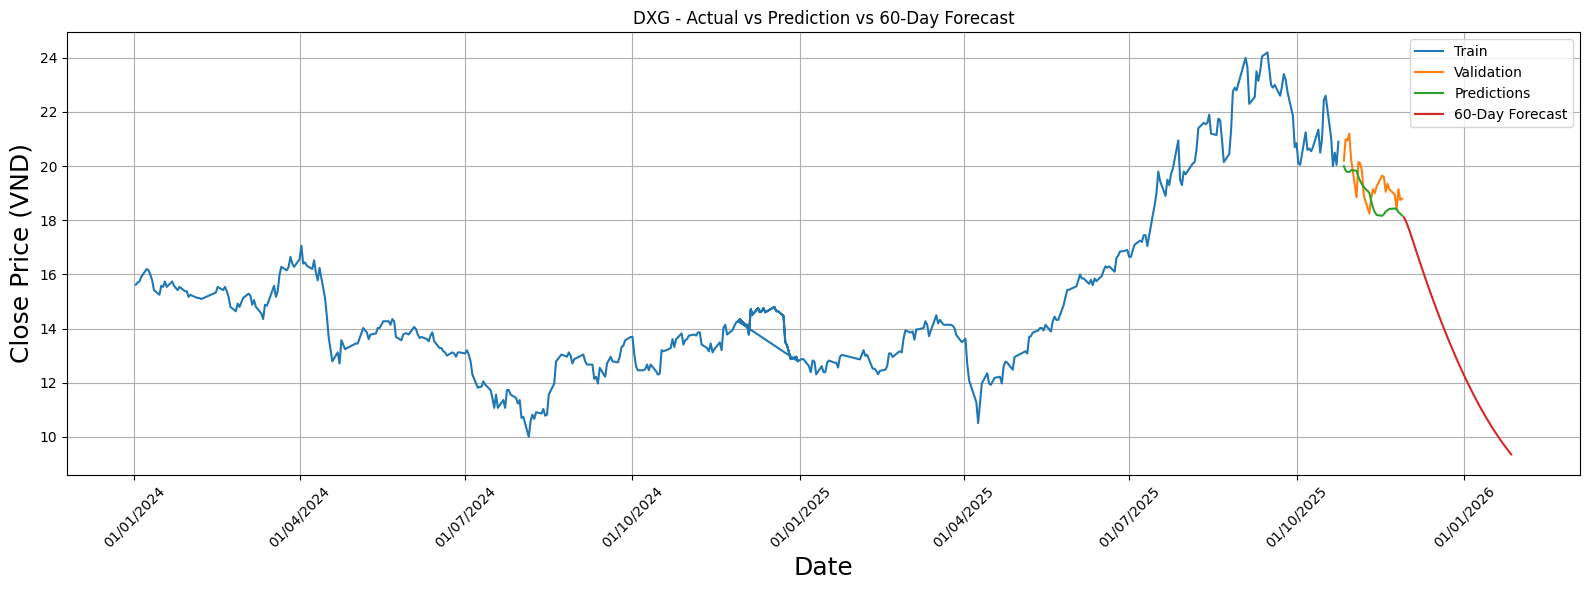
\includegraphics[width=\linewidth,height=4.0cm]{anh/singleagent/dxgagent.png}
        \caption{DXG}
        \label{fig:dxg}
    \end{subfigure}
    \hfill
    \begin{subfigure}[b]{0.48\columnwidth}
        \centering
        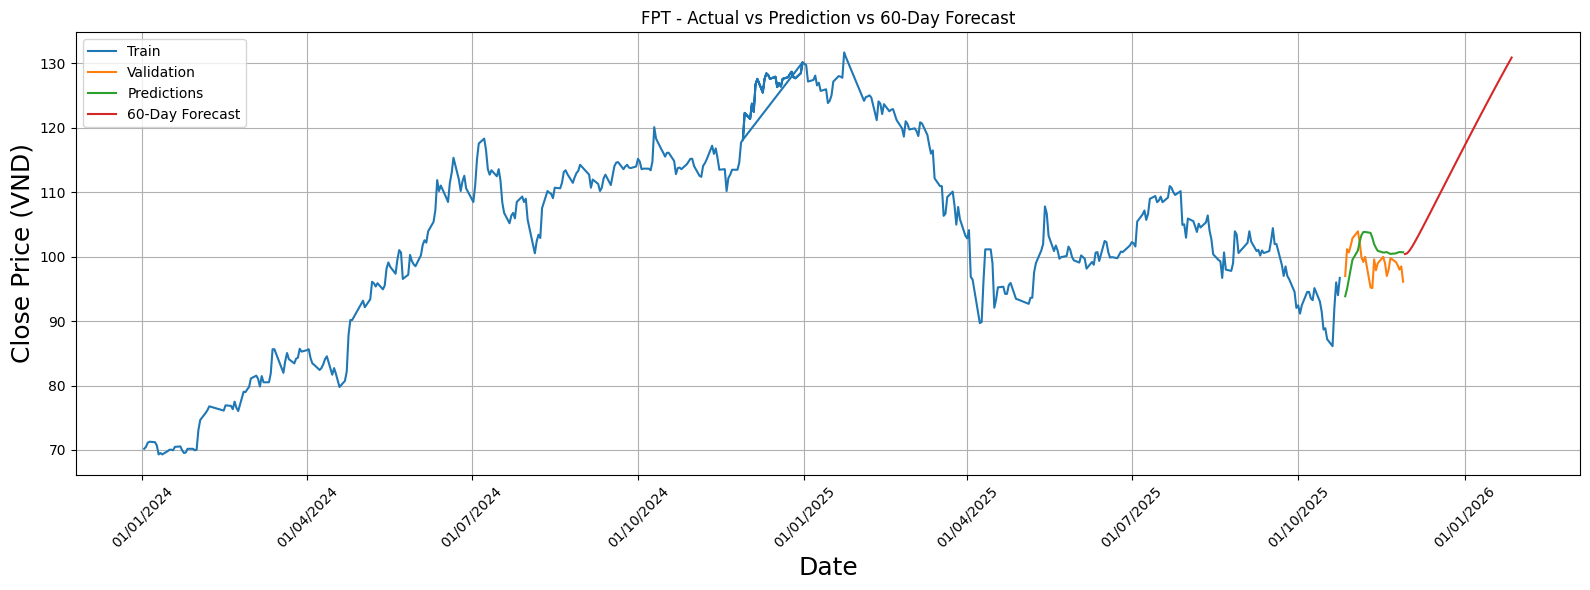
\includegraphics[width=\linewidth,height=4.0cm]{anh/singleagent/fptagent.png}
        \caption{FPT}
        \label{fig:fpt}
    \end{subfigure}

    \vspace{2mm} % khoảng cách giữa 2 hàng

    % Hàng 2
    \begin{subfigure}[b]{0.48\columnwidth}
        \centering
        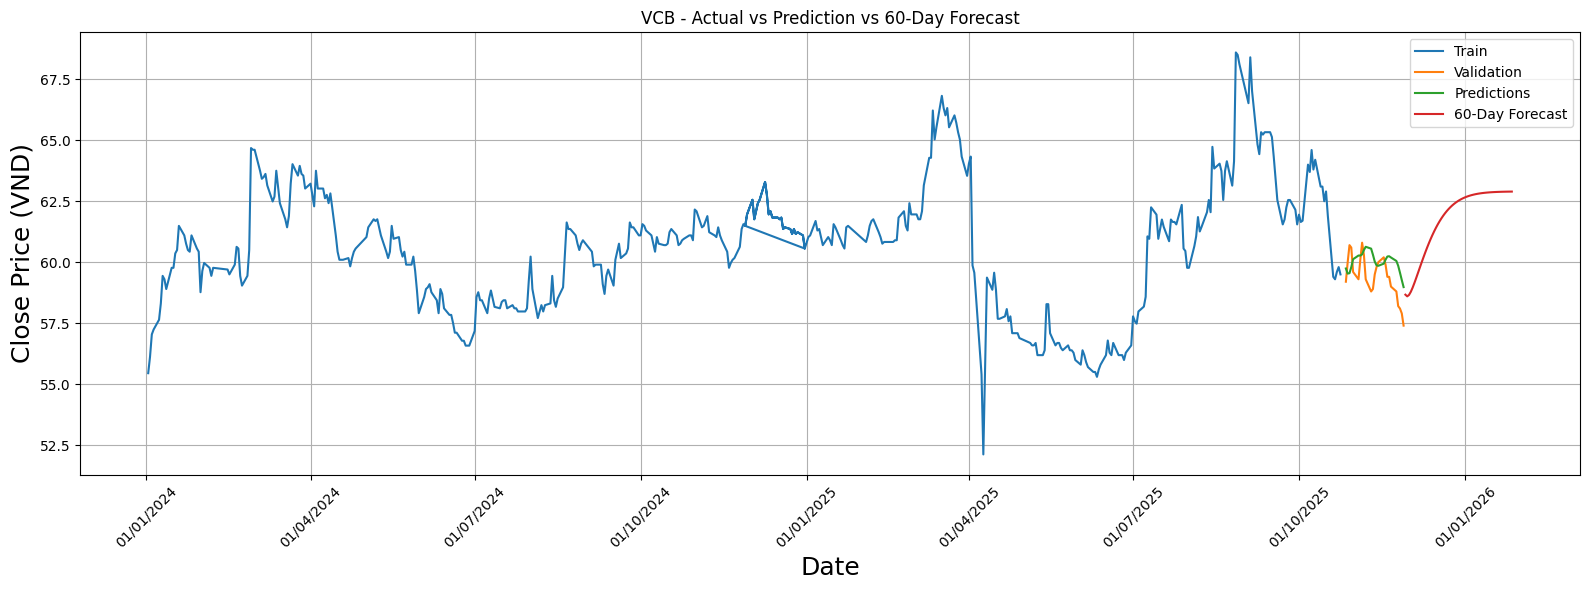
\includegraphics[width=\linewidth,height=4.0cm]{anh/singleagent/vcbagent.png}
        \caption{VCB}
        \label{fig:vcb}
    \end{subfigure}
    \hfill
    \begin{subfigure}[b]{0.48\columnwidth}
        \centering
        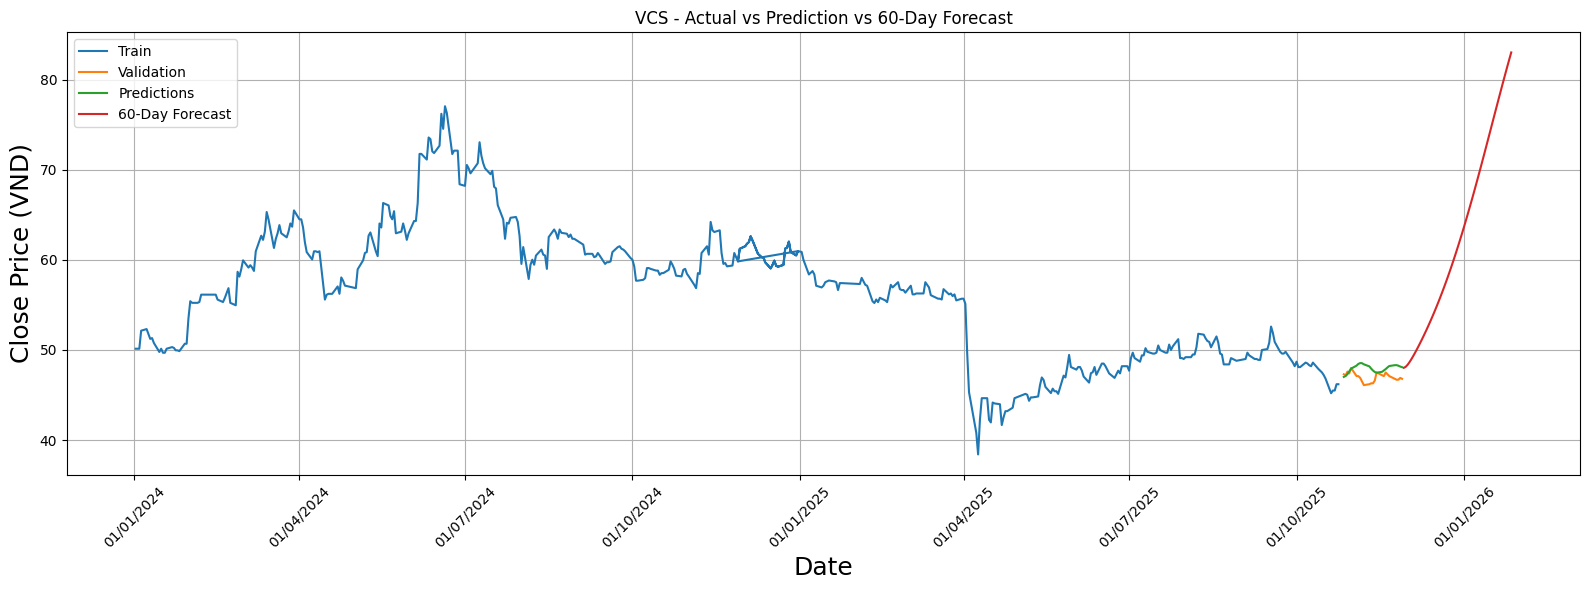
\includegraphics[width=\linewidth,height=4.0cm]{anh/singleagent/vcsagent.png}
        \caption{VCS}
        \label{fig:vcs}
    \end{subfigure}

    \caption{Result of 60-day forecast of Single-agent.}
    \label{fig:lstm_2x2}
\end{figure}

\clearpage
\onecolumn

\begin{table*}[!h]
\centering
\caption{Comparison of Short-term, Medium-term, and Long-term Forecasts Across Architectures and Stocks}
\label{tab:full_forecast}
\setlength{\tabcolsep}{3pt}
\renewcommand{\arraystretch}{1.05}
\scriptsize
\begin{tabular}{llcc|cccc|cccc|cccc}
\toprule
\multirow{2}{*}{\textbf{Stock}} &
\multirow{2}{*}{\textbf{Architecture}} &
\multicolumn{2}{c|}{\textbf{Start}} &
\multicolumn{4}{c|}{\textbf{Short-term}} &
\multicolumn{4}{c|}{\textbf{Medium-term}} &
\multicolumn{4}{c}{\textbf{Long-term}} \\
\cmidrule(lr){3-4}
\cmidrule(lr){5-8}
\cmidrule(lr){9-12}
\cmidrule(lr){13-16}
& &
\textbf{Date} & \textbf{Price} &
\textbf{End Date} & \textbf{Pred} & \textbf{Act} & \textbf{Gap} &
\textbf{End Date} & \textbf{Pred} & \textbf{Act} & \textbf{Gap} &
\textbf{End Date} & \textbf{Pred} & \textbf{Act} & \textbf{Gap} \\
\midrule


%%%%%%%%%%%%%%%%%%%%%%%%%%%%%%%%%%%%%%%%%%%%%%%%%%%%%%%%%%%%%%%%%%%%%%%%%%%%%%%%%%%%
% ===================== DXG ======================
%%%%%%%%%%%%%%%%%%%%%%%%%%%%%%%%%%%%%%%%%%%%%%%%%%%%%%%%%%%%%%%%%%%%%%%%%%%%%%%%%%%%
\multirow{4}{*}{\textbf{DXG}} 
& \textbf{Hierarchical}
& 31/08 & 22.8 & 03/09 & 22.25 & 24 & \textcolor{green}{\(\uparrow\)+1.75} & 14/09 & 23.38 & 24.05 & \textcolor{green}{\(\uparrow\) +0.67} & 30/10 & 21.83 & 21.2 &\textcolor{red}{\(\downarrow\) -0.63} \\

& 
& 16/10 & 22.45 & 19/10 & 22.10 & 22.6 & \textcolor{green}{\(\uparrow\)+0.5} & 30/10 & 23.34 & 21.2 & \textcolor{red}{\(\downarrow\) -2.14} & 15/12 & 24.46 & -- & -- \\

& 
& 21/10 & 20.0 & 24/10 & 20.51 & 20.9 & \textcolor{green}{\(\uparrow\)+0.39} & 04/11 & 20.52 & 20.15 & \textcolor{red}{\(\downarrow\) -0.37} & 20/12 & 20.81 & -- & -- \\

&
& 22/10 & 20.5 & 25/10 & 21.10 & 20.9 & \textcolor{red}{\(\downarrow\)-0.2}& 5/11 & 28.88 & 20.1 & \textcolor{red}{\(\downarrow\) -8.78} & 21/12 & 26.71 & -- & -- \\
\midrule


\multirow{4}{*}{\textbf{DXG}} 
& \textbf{Round Robin}
& 31/08 & 22.8 & 03/09 & 22.25 & 24 & \textcolor{green}{\(\uparrow\)+1.75} & 14/09 & 21.98 & 24.05 & \textcolor{red}{\(\downarrow\)-2.07} & 30/10 & 24.47 & 21.2 & \textcolor{red}{\(\downarrow\)-3.27} \\

&
& 16/10 & 22.45 & 19/10 & 22.15 & 22.6 & \textcolor{green}{\(\uparrow\)+0.45} & 30/10 & 22.28 & 21.2 & \textcolor{red}{\(\downarrow\)-1.08} & 15/12 & 25.63 & -- & -- \\

&
& 21/10 & 20.0 & 24/10 & 20.34 & 20.9 & \textcolor{green}{\(\uparrow\)+0.39} & 04/11 & 20.79 & 20.15 & 0.64 & 20/12 & 20.96 & -- & -- \\

&
& 22/10 & 20.5 & 25/10 & 20.48 & 20.9 & 0.42 & 05/11 & 23.68 & 20.1 & 3.58 & 21/12 & 26.71 & -- & -- \\
\midrule


\multirow{4}{*}{\textbf{DXG}} 
& \textbf{Ensemble}
& 31/08 & 22.8 & 03/09 & 22.11 & 24 & +1.75 & 14/09 & 22.98 & 24.05 & 1.07 & 30/10 & 21.47 & 21.2 & 0.27 \\

&
& 16/10 & 22.45 & 19/10 & 21.92 & 22.6 & \textcolor{green}{\(\uparrow\)+0.68} & 30/10 & 21.75 & 21.2 & \textcolor{red}{\(\downarrow\)-0.55} & 15/12 & 23.36 & -- & -- \\

&
& 21/10 & 20.0 & 24/10 & 20.07 & 20.9 & \textcolor{green}{\(\uparrow\)+0.83} & 04/11 & 20.52 & 20.15 & 0.37 & 20/12 & 20.81 & -- & -- \\

&
& 22/10 & 20.3 & 25/10 & 21.05 & 20.9 & +0.38 & 05/11 & 26.35 & 20.1 & 6.25 & 21/12 & -- & -- & -- \\
\midrule



%%%%%%%%%%%%%%%%%%%%%%%%%%%%%%%%%%%%%%%%%%%%%%%%%%%%%%%%%%%%%%%%%%%%%%%%%%%%%%%%%%%%
% ===================== FPT ======================
%%%%%%%%%%%%%%%%%%%%%%%%%%%%%%%%%%%%%%%%%%%%%%%%%%%%%%%%%%%%%%%%%%%%%%%%%%%%%%%%%%%%
\multirow{4}{*}{\textbf{FPT}} 
& \textbf{Hierarchical}
& 01/09 & 101.6 & 04/09 & 103.60 & 105 & \textcolor{green}{\(\uparrow\)+1.4} & 15/09 & 106.07 & 101.9 & -4.17 & 31/10 & 105.57 & 103.9 & 1.67 \\

&
& 16/10 & 89.8 & 19/10 & 90.83 & 88.1 & \textcolor{red}{\(\downarrow\)-2.73} & 30/10 & 89.32 & 102.7 & 13.38 & 15/12 & 92.13 & -- & -- \\

&
& 21/10 & 93 & 24/10 & 95.37 & 97.7 & \textcolor{green}{\(\uparrow\)+2.33} & 04/11 & 95.80 & 103.3 & \textcolor{green}{\(\uparrow\)+7.5} & 20/12 & 97.56 & -- & -- \\

&
& 22/10 & 97 & 25/10 & 93.5 & 97.7 & +4.2 & 05/11 & 97.60 & 100.9 & \textcolor{green}{\(\uparrow\)+3.3} & 21/12 & 108.92 & -- & -- \\
\midrule


\multirow{4}{*}{\textbf{FPT}} 
& \textbf{Round Robin}
& 01/09 & 101.6 & 03/09 & 104.42 & 105 & \textcolor{green}{\(\uparrow\)+0.58} & 15/09 & 105.66 & 101.9 & 3.76 & 31/10 & 104.27 & 103.9 & -- \\

&
& 16/10 & 127.5 & 19/10 & 127.9 & 129.1 & +1.2 & 01/11 & -- & -- & -- & 20/11 & -- & -- & -- \\

&
& 21/10 & 126.8 & 24/10 & 127.2 & 128.0 & +0.8 & 05/11 & -- & -- & -- & 25/11 & -- & -- & -- \\

&
& 25/10 & 126.2 & 25/10 & 126.8 & 127.7 & +0.9 & 10/11 & -- & -- & -- & 30/11 & -- & -- & -- \\
\midrule


\multirow{4}{*}{\textbf{FPT}} 
& \textbf{Ensemble}
& 31/08 & 128.0 & 03/09 & 129.3 & 130.5 & +1.2 & 15/09 & -- & -- & -- & 30/09 & -- & -- & -- \\

&
& 16/10 & 127.5 & 19/10 & 128.2 & 129.1 & +0.9 & 01/11 & -- & -- & -- & 20/11 & -- & -- & -- \\

&
& 21/10 & 126.8 & 24/10 & 127.5 & 128.0 & +0.5 & 05/11 & -- & -- & -- & 25/11 & -- & -- & -- \\

&
& 25/10 & 126.2 & 28/10 & 127.0 & 127.7 & +0.7 & 10/11 & -- & -- & -- & 30/11 & -- & -- & -- \\
\midrule




%%%%%%%%%%%%%%%%%%%%%%%%%%%%%%%%%%%%%%%%%%%%%%%%%%%%%%%%%%%%%%%%%%%%%%%%%%%%%%%%%%%%
% ===================== VCB ======================
%%%%%%%%%%%%%%%%%%%%%%%%%%%%%%%%%%%%%%%%%%%%%%%%%%%%%%%%%%%%%%%%%%%%%%%%%%%%%%%%%%%%
\multirow{4}{*}{\textbf{VCB}} 
& \textbf{Hierarchical}
& 31/08 & 92.3 & 03/09 & 92.8 & 93.5 & +0.7 & 15/09 & -- & -- & -- & 30/09 & -- & -- & -- \\

&
& 16/10 & 91.8 & 19/10 & 92.0 & 92.4 & +0.4 & 01/11 & -- & -- & -- & 20/11 & -- & -- & -- \\

&
& 21/10 & 91.5 & 24/10 & 91.9 & 92.1 & +0.2 & 05/11 & -- & -- & -- & 25/11 & -- & -- & -- \\

&
& 25/10 & 91.2 & 28/10 & 91.6 & 92.0 & +0.4 & 10/11 & -- & -- & -- & 01/12 & -- & -- & -- \\
\midrule


\multirow{4}{*}{\textbf{VCB}} 
& \textbf{Round Robin}
& 31/08 & 92.3 & 03/09 & 92.6 & 93.5 & +0.9 & 15/09 & -- & -- & -- & 30/09 & -- & -- & -- \\

&
& 16/10 & 91.8 & 19/10 & 91.9 & 92.4 & +0.5 & 01/11 & -- & -- & -- & 20/11 & -- & -- & -- \\

&
& 21/10 & 91.5 & 24/10 & 91.7 & 92.1 & +0.4 & 05/11 & -- & -- & -- & 25/11 & -- & -- & -- \\

&
& 25/10 & 91.2 & 28/10 & 91.5 & 92.0 & +0.5 & 10/11 & -- & -- & -- & 01/12 & -- & -- & -- \\
\midrule


\multirow{4}{*}{\textbf{VCB}} 
& \textbf{Ensemble}
& 31/08 & 92.3 & 03/09 & 92.9 & 93.5 & +0.6 & 15/09 & -- & -- & -- & 30/09 & -- & -- & -- \\

&
& 16/10 & 91.8 & 19/10 & 92.1 & 92.4 & +0.3 & 01/11 & -- & -- & -- & 20/11 & -- & -- & -- \\

&
& 21/10 & 91.5 & 24/10 & 91.9 & 92.1 & +0.2 & 05/11 & -- & -- & -- & 25/11 & -- & -- & -- \\

&
& 25/10 & 91.2 & 28/10 & 91.7 & 92.0 & +0.3 & 10/11 & -- & -- & -- & 01/12 & -- & -- & -- \\
\midrule



%%%%%%%%%%%%%%%%%%%%%%%%%%%%%%%%%%%%%%%%%%%%%%%%%%%%%%%%%%%%%%%%%%%%%%%%%%%%%%%%%%%%
% ===================== VCS ======================
%%%%%%%%%%%%%%%%%%%%%%%%%%%%%%%%%%%%%%%%%%%%%%%%%%%%%%%%%%%%%%%%%%%%%%%%%%%%%%%%%%%%
\multirow{4}{*}{\textbf{VCS}} 
& \textbf{Hierarchical}
& 31/08 & 45.2 & 03/09 & 45.5 & 46.1 & +0.6 & 15/09 & -- & -- & -- & 30/09 & -- & -- & -- \\

&
& 16/10 & 44.8 & 19/10 & 45.0 & 45.6 & +0.6 & 01/11 & -- & -- & -- & 20/11 & -- & -- & -- \\

&
& 21/10 & 44.5 & 24/10 & 44.7 & 45.0 & +0.3 & 05/11 & -- & -- & -- & 25/11 & -- & -- & -- \\

&
& 25/10 & 44.3 & 28/10 & 44.6 & 45.0 & +0.4 & 10/11 & -- & -- & -- & 01/12 & -- & -- & -- \\
\midrule


\multirow{4}{*}{\textbf{VCS}} 
& \textbf{Round Robin}
& 31/08 & 45.2 & 03/09 & 45.4 & 46.1 & +0.7 & 15/09 & -- & -- & -- & 30/09 & -- & -- & -- \\

&
& 16/10 & 44.8 & 19/10 & 44.9 & 45.6 & +0.7 & 01/11 & -- & -- & -- & 20/11 & -- & -- & -- \\

&
& 21/10 & 44.5 & 24/10 & 44.6 & 45.0 & +0.4 & 05/11 & -- & -- & -- & 25/11 & -- & -- & -- \\

&
& 25/10 & 44.3 & 28/10 & 44.5 & 45.0 & +0.5 & 10/11 & -- & -- & -- & 01/12 & -- & -- & -- \\
\midrule


\multirow{4}{*}{\textbf{VCS}} 
& \textbf{Ensemble}
& 31/08 & 45.2 & 03/09 & 45.6 & 46.1 & +0.5 & 15/09 & -- & -- & -- & 30/09 & -- & -- & -- \\

&
& 16/10 & 44.8 & 19/10 & 45.1 & 45.6 & +0.5 & 01/11 & -- & -- & -- & 20/11 & -- & -- & -- \\

&
& 21/10 & 44.5 & 24/10 & 44.8 & 45.0 & +0.2 & 05/11 & -- & -- & -- & 25/11 & -- & -- & -- \\

&
& 25/10 & 44.3 & 28/10 & 44.7 & 45.0 & +0.3 & 10/11 & -- & -- & -- & 01/12 & -- & -- & -- \\

\bottomrule
\end{tabular}
\end{table*}



\clearpage
\twocolumn
\bibliographystyle{IEEEtran}
\bibliography{refs}





\EOD
\end{document}
